\setcounter{chapter}{7}
\chapter{Simulation Analysis}
\label{cha:simulation_analysis}
% \minitoc
% 
% 
\section{Parameter narrowing}
% 
\TODO[inline]{siehe liste}
\begin{itemize}
    \item optical sigma
    \item sensor gain
    \item tilt angle
    \item micro oder macro -> simulation
    \item dn -> trel? different density?
    \item voxelsize -> simulation
    \item intensity/noise ->fixed with sigma noise
    \item LAP pixel size / which density, fiber configuration, ... can be identified
\end{itemize}
% 
% 
\subsection{predict/measure/literature parameters}
% 
\itodo{in prev chapter}
% 
\begin{figure}[!t]
\centering
\subcaptionbox{taorad pm. Line width: magenta: \SI{2.19}{\micro\meter}, yellow \SI{1.95}{\micro\meter} and cyan \SI{1.74}{\micro\meter}}[.49\textwidth]{
\begin{tikzpicture}
    \node[anchor=south east,inner sep=0] at (0,0) {
    \scalebox{-1}[1]{\includegraphics[width=0.49\textwidth, trim = 919 1205 1029 743, clip, interpolate=false, ]{data/Taorad_USAF_AB4_LB85_5pct_5ms_a00_t000_1.png}}};
\begin{scope}[xscale=-1]
    \draw[magenta,ultra thick,rounded corners] (0.25,0.5) rectangle (1.5,1.25);
    \draw[yellow,ultra thick,rounded corners] (2,0.75) rectangle (3.15,1.5);
    \draw[cyan,ultra thick,rounded corners] (3.0,2.3) rectangle (3.9,2.8);
    % \draw[green,ultra thick] (0,0) grid (5,5);
\end{scope}
\end{tikzpicture}
}%\hfill
% \subcaptionbox{retardation}[.49\textwidth]{
% \includegraphics[width=0.49\textwidth]{dev/gfx/2/retardation.pdf}}
\caption{USAF}
\label{fig:USAF}
\end{figure}

% 
\begin{figure}[!t]
\centering
\subcaptionbox{transmittance}[.49\textwidth]{
\includegraphics[width=0.49\textwidth]{dev/gfx/2/transmittance_PM_Vervet.pdf}}\hfill
\subcaptionbox{retardation}[.49\textwidth]{
\includegraphics[width=0.49\textwidth]{dev/gfx/2/retardation_PM_Vervet.pdf}}
\caption{Flat model simulations}
\label{fig:parameterModelSim}
\end{figure}
% 
To simulate \ac{3D-PLI} with nerve fiber models as realistic as possible specific parameters for the absorption and birefringence has to be choosen.
From the literatur the birefringence of \ac{WM} nerve fibers lies around \dummy{}.
However since the nerve fiber models are stiff, the density of myelin in a section will be most probably lower then in the experiments.
To be able to predict the influence of noice it was decided to increase the birefringence on a level, so that the retardation value reaches a reasonable value.
\\
Looking for the human tissue section \cref{fig:human:transmittance} one can see, that the retardation value does not over 0.83\todo{retardation in PM higher, but not in homogenious regions}.
This is choices by the tissue section, so that the signal as described in \dummy{} is not \dummy{}.
A reagion with very high retardation, and therefore most probably flat fibers, has values about $\SI{0.71\pm0.02}{}$.
To reach these values for a flat dense mode one has to set the birefringence to $\SI{-0.003}{}$ or $\SI{0.006}{}$ depending on the chosen model \cref{fig:parameterModelSim}. Higher values lead for large fiber radii to \dummy{}. This is still in the range of the literature \dummy{} \todo{check again}.
% 
% 
\paragraph{intensity}
% 
multiple images, background, 
LAP-> ...
PM -> ...
% 
\paragraph{gratio}
% 
\begin{figure}[!t]
\centering
\subcaptionbox{transmittance}[.49\textwidth]{
\includegraphics[width=0.49\textwidth]{dev/gfx/2/LAP_noise.png}}\hfill
\subcaptionbox{retardation}[.49\textwidth]{
\includegraphics[width=0.49\textwidth]{dev/gfx/2/PM_noise.png}}
\caption{Flat model simulations}
\label{fig:parameterModelSim}
\end{figure}
% 
% X
\paragraph{birefringence}
\cref{fig:brain_ret}
% 
\paragraph{absorption}
\cref{fig:brain_trans}
% 
\paragraph{artificial downsampling}
Analog to \cite{Menzel:155964} - 5.1.3.2 Artificial Downsampling, the optical resolution wa sdetermand for the different experimental setups:
0.7 LAP, 0.78 PM, 0.84 Taorad. (only 0.75 is used)
% 
% 
\begin{figure}[!t]
\captionsetup[sub]{position=top}
\subcaptionbox{\label{fig:human:transmittance}}[0.84\textwidth]{
% \fbox{
\begin{tikzpicture}[trim axis left, trim axis right]
\begin{axis}[%
width=0.84\textwidth,
% title = {$B_1^{equ}$ in $\mu T$},
xmin=0.5,xmax=1525.5,ymin=0.5,ymax=995.5,y dir=reverse,
point meta min=6567,point meta max=14085,
hide axis,
colormap/blackwhite,colorbar,
]
\addplot [forget plot] graphics [xmin=0.5,xmax=1525.5,ymin=0.5,ymax=995.5] {dev/gfx/data/MSA0309_M8_70mu_70ms_s0666_a00_d000_Transmittance.png};
\end{axis}
\end{tikzpicture}
\label{fig:brain_trans}
}
\\[2em]
\subcaptionbox{}[0.84\textwidth]{
\begin{tikzpicture}[trim axis left, trim axis right]
\begin{axis}[%
width=0.84\textwidth,
% title = {$B_1^{equ}$ in $\mu T$},
xmin=0.5,xmax=1525.5,ymin=0.5,ymax=995.5,y dir=reverse,
point meta min=0,point meta max=0.8377,
hide axis,
colormap/blackwhite,colorbar,
]
\addplot [forget plot] graphics [xmin=0.5,xmax=1525.5,ymin=0.5,ymax=995.5] {dev/gfx/data/MSA0309_M8_70mu_70ms_s0666_a00_d000_Retardation.png};
\end{axis}
\end{tikzpicture}
\label{fig:brain_ret}
}\hspace*{\fill}
 \caption[]{\dummy{} human brain}
\label{fig:brain_ret_trans}
\end{figure}
% 
% 
% 
% 
% 
\section{voxel size}
% 
% ../../1_model/1_cubes/output/cube_2pop_120/cube_2pop_psi_1.00_omega_0.00_r_5.00_v0_120_.solve[65/927]
% 0 [1536] [0] [-6. -6.] [ 4  4 96] [ -6.  -6. -30.]
% /data/PLI-Group/felix/data/thesis/env-ime263/lib/python3.6/site-packages/fastpli/simulation/_simpli.p
% y:76: UserWarning: All labels are 0. Usually this means, that the VOI contains no
%  fiber_bundles or that the voxel_size is to large.
%   UserWarning)
% ../../1_model/1_cubes/output/cube_2pop_120/cube_2pop_psi_1.00_omega_0.00_r_5.00_v0_120_.solved.h5 90
% 0 [1536] [0] [-6. -6.] [ 4  4 96] [ -6.  -6. -30.]
% /data/PLI-Group/felix/data/thesis/env-ime263/lib/python3.6/site-packages/fastpli/simulation/_simpli.p
% y:76: UserWarning: All labels are 0. Usually this means, that the VOI contains no
%  fiber_bundles or that the voxel_size is to large.
%   UserWarning)
% ../../1_model/1_cubes/output/cube_2pop_120/cube_2pop_psi_1.00_omega_0.00_r_5.00_v0_120_.solved.h5 90
% 0 [1536] [0] [-6. -6.] [ 4  4 96] [ -6.  -6. -30.]
% /data/PLI-Group/felix/data/thesis/env-ime263/lib/python3.6/site-packages/fastpli/simulation/_simpli.p
% y:76: UserWarning: All labels are 0. Usually this means, that the VOI contains no
%  fiber_bundles or that the voxel_size is to large.
%   UserWarning)
% ../../1_model/1_cubes/output/cube_2pop_120/cube_2pop_psi_1.00_omega_0.00_r_5.00_v0_120_.solved.h5 90
% 0 [1536] [0] [-6. -6.] [ 4  4 96] [ -6.  -6. -30.]
% /data/PLI-Group/felix/data/thesis/env-ime263/lib/python3.6/site-packages/fastpli/simulation/_simpli.p
% y:76: UserWarning: All labels are 0. Usually this means, that the VOI contains no
%  fiber_bundles or that the voxel_size is to large.
%   UserWarning)
% ../../1_model/1_cubes/output/cube_2pop_120/cube_2pop_psi_1.00_omega_0.00_r_5.00_v0_120_.solved.h5 90
% 0 [192] [0] [-6. -6.] [ 2  2 48] [ -6.  -6. -30.]
% /data/PLI-Group/felix/data/thesis/env-ime263/lib/python3.6/site-packages/fastpli/simulation/_simpli.p
% y:76: UserWarning: All labels are 0. Usually this means, that the VOI contains no
%  fiber_bundles or that the voxel_size is to large.
%   UserWarning)
% ../../1_model/1_cubes/output/cube_2pop_120/cube_2pop_psi_1.00_omega_0.00_r_5.00_v0_120_.solved.h5 90
% 0 [192] [0] [-6. -6.] [ 2  2 48] [ -6.  -6. -30.]
% /data/PLI-Group/felix/data/thesis/env-ime263/lib/python3.6/site-packages/fastpli/simulation/_simpli.p
% y:76: UserWarning: All labels are 0. Usually this means, that the VOI contains no
%  fiber_bundles or that the voxel_size is to large.
%   UserWarning)
% ../../1_model/1_cubes/output/cube_2pop_120/cube_2pop_psi_1.00_omega_0.00_r_5.00_v0_120_.solved.h5 90
% 0 [192] [0] [-6. -6.] [ 2  2 48] [ -6.  -6. -30.]
% /data/PLI-Group/felix/data/thesis/env-ime263/lib/python3.6/site-packages/fastpli/simulation/_simpli.p
% y:76: UserWarning: All labels are 0. Usually this means, that the VOI contains no
%  fiber_bundles or that the voxel_size is to large.
%   UserWarning)
% ../../1_model/1_cubes/output/cube_2pop_120/cube_2pop_psi_1.00_omega_0.00_r_5.00_v0_120_.solved.h5 90
% 0 [192] [0] [-6. -6.] [ 2  2 48] [ -6.  -6. -30.]
% /data/PLI-Group/felix/data/thesis/env-ime263/lib/python3.6/site-packages/fastpli/simulation/_simpli.p
% y:76: UserWarning: All labels are 0. Usually this means, that the VOI contains no
%  fiber_bundles or that the voxel_size is to large.
%   UserWarning)
% ../../1_model/1_cubes/output/cube_2pop_120/cube_2pop_psi_1.00_omega_0.00_r_5.00_v0_120_.solved.h5 90
% 0 [192] [0] [-6. -6.] [ 2  2 48] [ -6.  -6. -30.]
% /data/PLI-Group/felix/data/thesis/env-ime263/lib/python3.6/site-packages/fastpli/simulation/_simpli.p
% y:76: UserWarning: All labels are 0. Usually this means, that the VOI contains no
%  fiber_bundles or that the voxel_size is to large.
%   UserWarning)
% ../../1_model/1_cubes/output/cube_2pop_120/cube_2pop_psi_1.00_omega_0.00_r_5.00_v0_120_.solved.h5 90
% 0 [192] [0] [-6. -6.] [ 2  2 48] [ -6.  -6. -30.]

% 
\begin{figure}[!t]
\centering
\resizebox{1.0\textwidth}{!}{
\tikzset{external/export=false}
\definecolor{c1}{rgb}{0.25,0.4,0.1}
\definecolor{c2}{rgb}{1.0,0.73,0}
\definecolor{c3}{rgb}{0.98,0.4,0.25}
\definecolor{c4}{rgb}{0.22,0.36,0.59}
%
% \definecolor{c1}{HTML}{440154FF}
% \definecolor{c2}{HTML}{38598CFF}
% \definecolor{c3}{HTML}{1E9B8AFF}
% \definecolor{c4}{HTML}{FDE725FF}
%
\def\xc{0.7}
\def\yc{0.2}
\def\rin{1.5}
\def\rout{3}
%
% 
\newcommand{\fiber}[3]{
	\def\dd{#1}
	\pgfmathsetmacro{\xmin}{int(floor(\xc-\rout))}
	\pgfmathsetmacro{\xmax}{int(ceil(\xc+\rout))}
	\pgfmathsetmacro{\xd}{\xmin+\dd}
	\pgfmathsetmacro{\ymin}{int(floor(\yc-\rout))}
	\pgfmathsetmacro{\ymax}{int(ceil(\yc+\rout))}
	\pgfmathsetmacro{\yd}{\ymin+\dd}
	%
	\pgfmathsetmacro{\rmin}{\rin*\rin*100}
	\pgfmathsetmacro{\rmax}{\rout*\rout*100}
	\foreach \x in {\xmin,\xd,...,\xmax} {
		\foreach \y in {\ymin,\yd,...,\ymax} {
			\pgfmathsetmacro{\d}{int(((\x-\xc+\dd/2)*(\x-\xc+\dd/2)+(\y-\yc+\dd/2)*(\y-\yc+\dd/2))*100)}
			\ifnum\d>\rmin
			\ifnum\d<\rmax
			\path [#3] (\x,\y) rectangle ($ (\x, \y) + (\dd, \dd) $);
			\draw[#2] ($ (\x, \y) + (0, 0) $) -- ($ (\x, \y) + (\dd, 0) $);
			\draw[#2] ($ (\x, \y) + (\dd, 0) $) -- ($ (\x, \y) + (\dd, \dd) $);
			\draw[#2] ($ (\x, \y) + (\dd, \dd) $) -- ($ (\x, \y) + (0, \dd) $);
			\draw[#2] ($ (\x, \y) + (0, \dd) $) -- ($ (\x, \y) + (0, 0) $);
			\fi\fi
		}
	}
%	\foreach \x in {\xmin,\xd,...,\xmax} {
%		\draw[#2] (\x,\ymin) -- (\x,\ymax);
%	}
%	\foreach \y in {\ymin,\yd,...,\ymax} {
%		\draw[#2] (\xmin,\y) -- (\xmax,\y);
%	}
}
%
\subcaptionbox{}[\tikzwidth]{
\resizebox{\tikzwidth}{!}{
\begin{tikzpicture}[]
\path[] (-3.75, -3.5) rectangle (3.75, 3.25);
\begin{scope}[shift={(-\xc,-\yc)}]
\fiber{2}{line width = 0.2mm}{pattern color=c1,pattern=horizontal lines}
\draw[line width = 0.4mm] (\xc,\yc) circle (\rin);
\draw[line width = 0.4mm] (\xc,\yc) circle (\rout);
\end{scope}
\end{tikzpicture}
}}
\hfill
%
\subcaptionbox{}[\tikzwidth]{
\resizebox{\tikzwidth}{!}{
\begin{tikzpicture}[]
\path[] (-3.75, -3.5) rectangle (3.75, 3.25);
\begin{scope}[shift={(-\xc,-\yc)}]
\fiber{1}{line width = 0.1mm}{pattern color=c2,pattern=vertical lines}
\draw[line width = 0.4mm] (\xc,\yc) circle (\rin);
\draw[line width = 0.4mm] (\xc,\yc) circle (\rout);
\end{scope}
\end{tikzpicture}
}}
\hfill
%
\subcaptionbox{}[\tikzwidth]{
\resizebox{\tikzwidth}{!}{
\begin{tikzpicture}[]
\path[] (-3.75, -3.5) rectangle (3.75, 3.25);
\begin{scope}[shift={(-\xc,-\yc)}]
\fiber{0.5}{line width = 0.05mm}{pattern color=c3,pattern=north east lines}
\draw[line width = 0.4mm] (\xc,\yc) circle (\rin);
\draw[line width = 0.4mm] (\xc,\yc) circle (\rout);
\end{scope}
\end{tikzpicture}
}}
\hfill
%
\subcaptionbox{}[\tikzwidth]{
\resizebox{\tikzwidth}{!}{
\begin{tikzpicture}[]
\path[] (-3.75, -3.5) rectangle (3.75, 3.25);
\begin{scope}[shift={(-\xc,-\yc)}]
\fiber{0.25}{line width = 0.025mm}{pattern color=c4,pattern=crosshatch dots}
\draw[line width = 0.4mm] (\xc,\yc) circle (\rin);
\draw[line width = 0.4mm] (\xc,\yc) circle (\rout);
\end{scope}
% \fiber{2}{}{fill, c1, opacity=0.25}
% \fiber{1}{very thin}{fill, c2, opacity=0.25}
% \fiber{0.5}{ultra thin}{fill, c3, opacity=0.25}
% \fiber{0.25}{ultra thin}{fill, c4, opacity=0.25}
%
\end{tikzpicture}
}}}
\caption[Discretization error]{Discretization error.
This behavior is much stronger with myelin layers}
\label{fig:vectorfield_disc_error}
\end{figure}
% 
\begin{figure}[p]
\centering
\includegraphics[width=\textwidth, page=4]{dev/gfx/2/voxel_size_plots_data_0.pdf}
\caption[]{\dummy{}}
\label{fig:voxelsize}
\end{figure}
% 
\begin{figure}[p]
\centering
\includegraphics[width=\textwidth, page=4]{dev/gfx/2/voxel_size_plots_data_1.pdf}
\caption[]{\dummy{}}
\label{fig:voxelsize}
\end{figure}
% 
% 
% 
% % \begin{figure}[!tbh]
% %     \centering
% %     \resizebox{.95\textwidth}{!}{
% %     % \inputtikz{gfx/test}
% %     }
% % 	\caption{test_plot}
% % 	\label{fig:test_plot}
% % \end{figure}
% % 

% \subsection{single fiber f}
% \begin{align*}
%     f(\alpha, \varphi) &= f(-\alpha, \varphi + \pi)\\
%     f(\alpha, \varphi) &= f(\alpha+2\pi, \varphi)  = f(\alpha, \varphi+2\pi)\\
% \end{align*}
% \begin{align*}
%     S:(f(\alpha, \varphi)) \rightarrow (\mathbb{R}, [0, 2 \pi), [0, 1)))\\
%     S(f(\alpha, \varphi)) = S(f(\alpha, \varphi - \Delta\varphi)) + \begin{pmatrix}0\\ \Delta \varphi\\ 0\end{pmatrix}\\
%     S(T(f(\alpha, \varphi), \theta, \phi) = S(T(f(\alpha+, \varphi+), -\theta, -\phi)
% \end{align*}
% % 
% \subsection{two fiber population}
% \begin{align*}
%     S(f_0(\alpha, \varphi), f_1(\omega, \psi)) = \\
%     T(S(f_0(\alpha, \varphi), f_1(\omega, \psi)), \theta, \phi) = 
% \end{align*}
% % 
% % \begin{figure}[!t]
% % \centering
% % \def\tikzwidth{0.45*\textwidth}
% % \subcaptionbox{...}[.49\textwidth]{
% % \inputtikz{gfx/model/sphere_models_a}}
% % \subcaptionbox{...}[.49\textwidth]{
% % \inputtikz{gfx/model/sphere_models_b}}
% % \caption{...}
% % \end{figure}
% % 
% \subsection{simulation sampling}
% % 
% \begin{itemize}
%     \item \micro or \macro
%     \item \voxelsize
% \end{itemize}

% to identify the needed optical resolution inside the simulation, the \voxelsize and \model(\micro or \macro) will be analysed.
% The question is, how big can the \voxelsize be so that the resulting signal (for one \ac{PM} pixel) is not significantly different.
% The same is true for the choice of \model.
% The simulation setup is as follows:

% \begin{table}[!b]
% \centering
% \pgfplotstabletypeset[
%     column type=l,
%     every even row/.style={before row={\rowcolor[gray]{0.95}}},
%     columns/variable/.style={string type},
%     columns/value/.style={string type},
%     every head row/.style={before row=\toprule,after row=\midrule},
%     every last row/.style={after row=\bottomrule},
%     col sep=&,
%     row sep=\\,
% ]
% {variable & value\\
% simpli.pixel\_size & \SI{1.25}{\micro\meter}\\
% simpli.sensor\_gain & \SI{1.5}{}\\
% simpli.optical\_sigma & \SI{0.71}{}\\
% % simpli.filter\_rotations & np.linspace(0, np.pi, 9, False)\\
% simpli.interpolate & \SI{1}{}\\
% simpli.untilt\_sensor\_view & \SI{1}{}\\
% simpli.wavelength & \SI{525}{\nano\meter}  \\
% simpli.light\_intensity & \SI{50000}{\arbitraryunit} \\
% % simpli.tilts & \SI{np.deg2rad(np.array([(0, 0)]))}{}\\
% simpli.voxel\_size & \$\voxelsize\\
% % \multirow{2}{*}{simpli.set\_voi} & $-\SIlist[list-units = brackets,list-final-separator={, },]{0.5;0.5;30}{\micro\meter}$\\
% simpli.set\_voi & $-\SIlist[list-units = brackets,list-final-separator={, },]{0.5;0.5;30}{\micro\meter}$\\
% & $\phantom{-}\SIlist[list-units = brackets,list-final-separator={, },]{0.5;0.5;30}{\micro\meter}$\\
% }
% \caption{simulation setup}
% \end{table}
% % 
% % 
% % \begin{lstfloat}[!tb]
% % \lstset{
% % language=python,
% % keywordstyle=\color{blue},
% % stringstyle=\color{red},
% % commentstyle=\color{green!60!black},
% % tabsize=2
% % }
% % \begin{lstlisting}
% % PIXEL_SIZE = 1.0
% % FIBER_RADII = 1.0
% % THICKNESS = 60

% % simpli.pixel_size = PIXEL_SIZE
% % simpli.sensor_gain = 1.5  # in micro meter
% % simpli.optical_sigma = 0.71  # in voxel size
% % simpli.filter_rotations = np.linspace(0, np.pi, 9, False)
% % simpli.interpolate = True
% % simpli.untilt_sensor_view = True
% % simpli.wavelength = 525  # in nm
% % simpli.light_intensity = 50000  # a.u.
% % simpli.tilts = np.deg2rad(np.array([(0, 0)]))
% % simpli.voxel_size = voxel_size
% % simpli.set_voi(-0.5 * np.array([PIXEL_SIZE, PIXEL_SIZE, THICKNESS]),
% %               0.5 * np.array([PIXEL_SIZE, PIXEL_SIZE, THICKNESS]))
% % simpli.dim_origin = [10, 10, -0.5 * THICKNESS]
% % \end{lstlisting}
% % \label{alg:voxel_size_setup}
% % \caption{voxel\_size\_setup}
% % \end{lstfloat}
% % 
% % 
% % \begin{figure}[!t]
% %     \resizebox{\textwidth}{!}{
% %     \inputtikz{gfx/model/sphere_discretization}
% %     }
% % 	\caption{sphere\_discretization}
% % 	\label{fig:sphere_discretization}
% % \end{figure}
% % % 
% % \begin{figure}[!t]
% %     \resizebox{\textwidth}{!}{
% %     \inputtikz{data/5/voxel_size_vs_diff_dir}
% %     }
% % 	\caption{voxel\_size\_vs\_diff\_dir}
% % 	\label{fig:voxel_size_vs_diff_dir}
% % \end{figure}
% % 
% %  MACHT PROBLEME FIXME:
% % \begin{figure}[!t]
% %     \resizebox{\textwidth}{!}{
% %     \inputtikz{data/5/voxel_size_vs_retardation}
% %     }
% % 	\caption{voxel\_size\_vs\_retardation}
% % 	\label{fig:voxel_size_vs_retardation}
% % \end{figure}
% % 
% % \begin{figure}[!t]
% % \resizebox{\textwidth}{!}{
% % 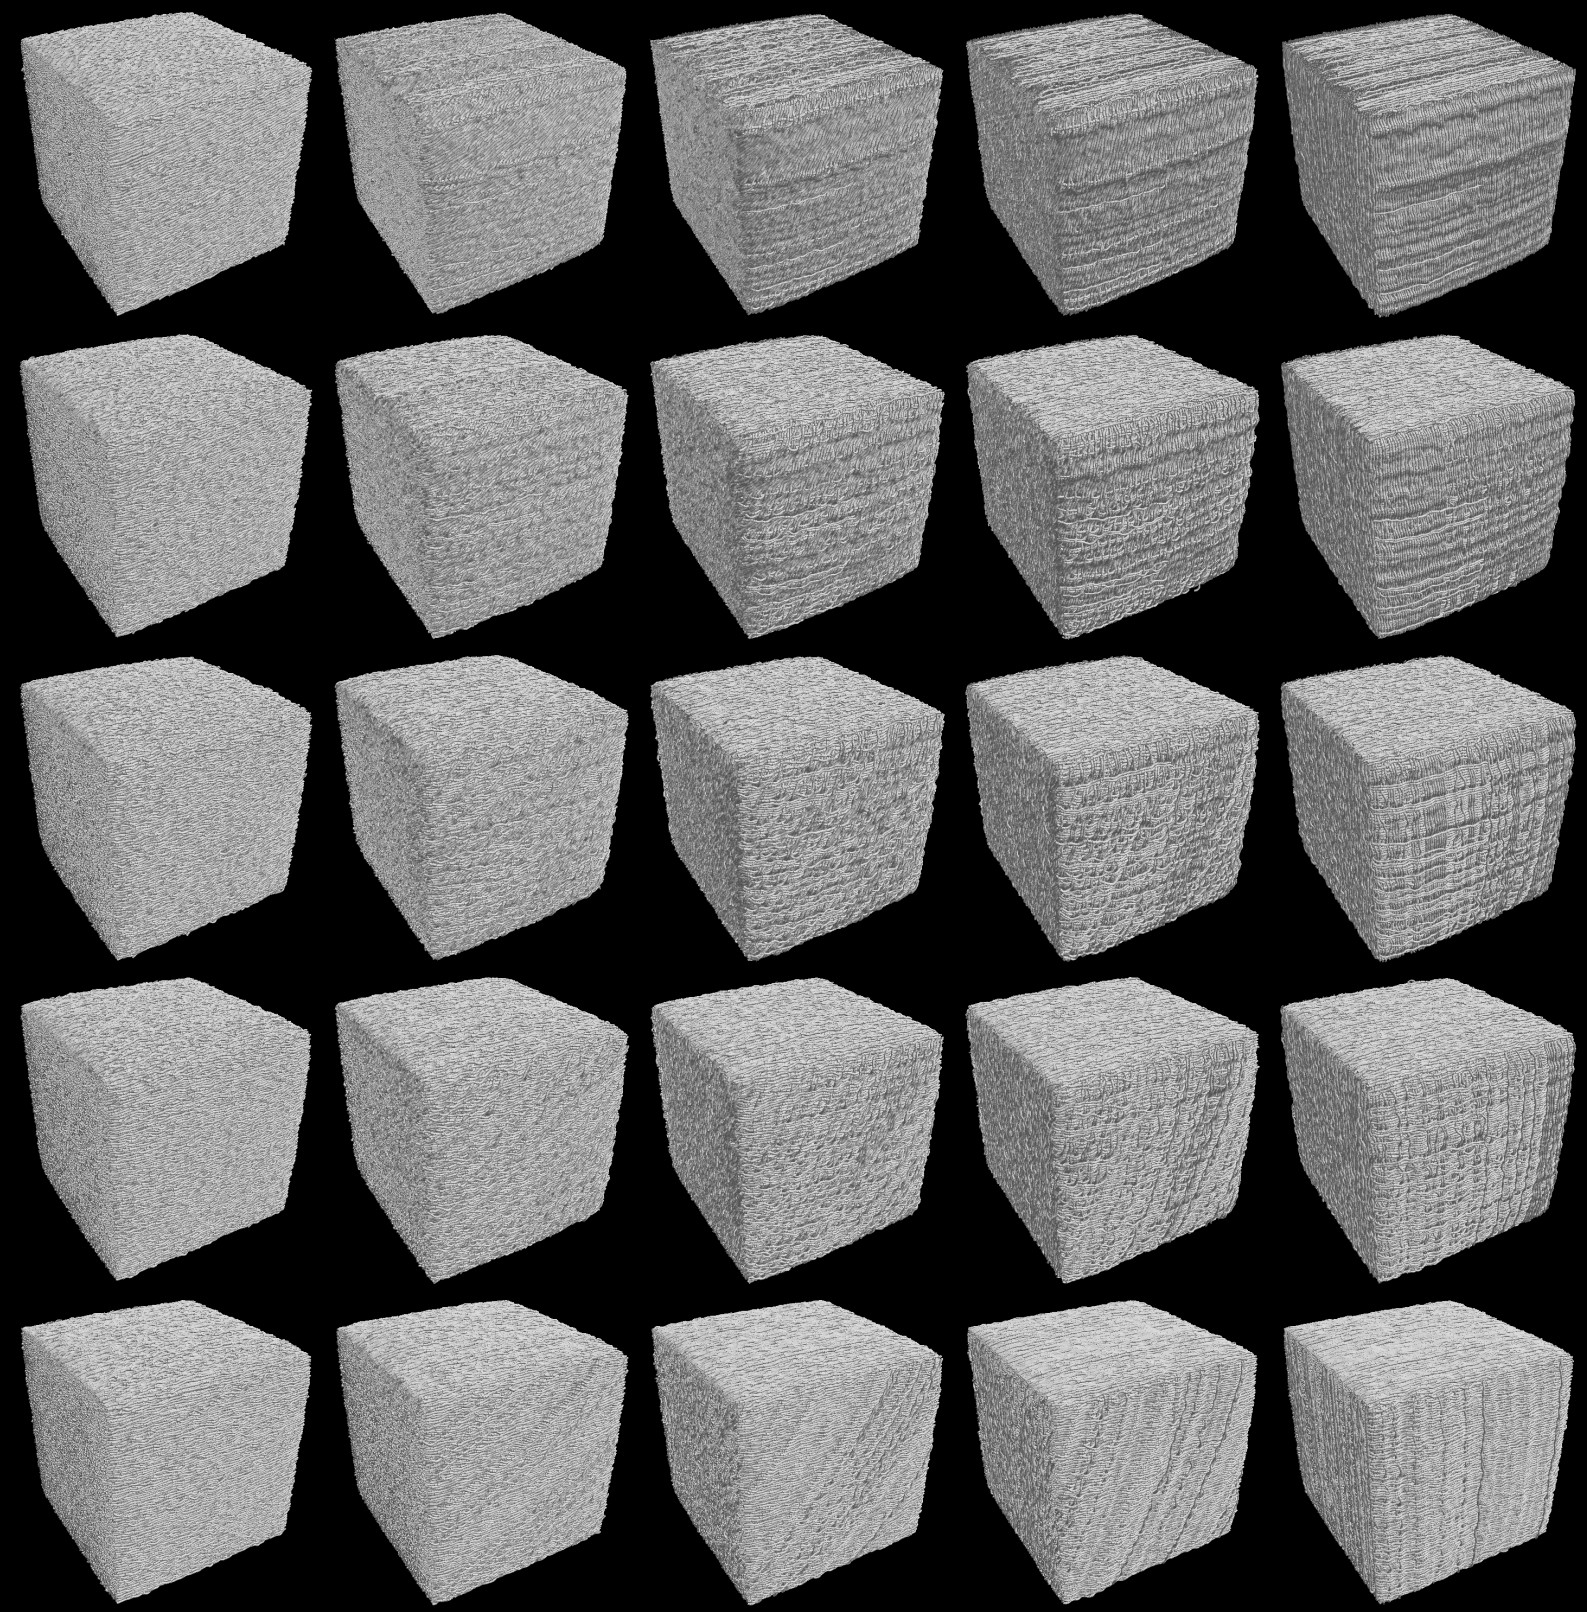
\includegraphics[]{gfx/model/cube_2pop_montage.jpg}
% % %\begin{minipage}{30cm}
% % %%\foreach \psi [count=\i] in {0.1, 0.2, 0.3, 0.4, 0.5, 0.6, 0.7, 0.8, 0.9}{
% % %%	\foreach \omega in {0.0, 10.0, 20.0, 30.0, 40.0, 50.0, 60.0, 70.0, 80.0, 90.0}{	
% % %\foreach \psi [count=\i] in {0.1, 0.3, 0.5, 0.7, 0.9}{
% % %    \foreach \omega in {10.0, 30.0, 50.0, 70.0, 90.0}{
% % %        \includegraphics[trim={110, 70, 90, 130}, clip, width=6cm] %width=2.5cm
% % %        {dev/data/cube_2pop/cube_2pop_psi_\psi_omega_\omega_.solved.ppm.png}
% % %        \hspace{-0.5cm}
% % %    }
% % %    \vspace{-0.1cm}
% % %    \ifthenelse{\i<9}{\newline}{}
% % %}
% % %\end{minipage}
% % }
% % \caption{A test}
% % \end{figure}
% % 
% % 
% % 
% % TODO:
% % \begin{figure}[!t]
% % \resizebox{\textwidth}{!}{
% % \foreach \omega in {0,30,60,90} {
% %     \resizebox{0.215\textwidth}{!}{
% %     \input{dev/data/pm_omega_\omega.0_psi_epa_dir.tikz}
% %     }
% % }}
% % \resizebox{\textwidth}{!}{
% % \foreach \omega in {0,30,60,90} {
% %     \resizebox{0.215\textwidth}{!}{
% %     \input{dev/data/pm_omega_\omega.0_psi_epa_ret.tikz}
% %     }
% % }}
% % \caption{A test}
% % \end{figure}

% % 
% \section{Optimal Grid Size}

% \subsection{Impact on labelfield}
% % 
% \begin{figure}[!t]
% \centering
% \resizebox{1.0\textwidth}{!}{
% \tikzset{external/export=false}
% \definecolor{c1}{rgb}{0.25,0.4,0.1}
\definecolor{c2}{rgb}{1.0,0.73,0}
\definecolor{c3}{rgb}{0.98,0.4,0.25}
\definecolor{c4}{rgb}{0.22,0.36,0.59}
%
% \definecolor{c1}{HTML}{440154FF}
% \definecolor{c2}{HTML}{38598CFF}
% \definecolor{c3}{HTML}{1E9B8AFF}
% \definecolor{c4}{HTML}{FDE725FF}
%
\def\xc{0.7}
\def\yc{0.2}
\def\rin{1.5}
\def\rout{3}
%
% 
\newcommand{\fiber}[3]{
	\def\dd{#1}
	\pgfmathsetmacro{\xmin}{int(floor(\xc-\rout))}
	\pgfmathsetmacro{\xmax}{int(ceil(\xc+\rout))}
	\pgfmathsetmacro{\xd}{\xmin+\dd}
	\pgfmathsetmacro{\ymin}{int(floor(\yc-\rout))}
	\pgfmathsetmacro{\ymax}{int(ceil(\yc+\rout))}
	\pgfmathsetmacro{\yd}{\ymin+\dd}
	%
	\pgfmathsetmacro{\rmin}{\rin*\rin*100}
	\pgfmathsetmacro{\rmax}{\rout*\rout*100}
	\foreach \x in {\xmin,\xd,...,\xmax} {
		\foreach \y in {\ymin,\yd,...,\ymax} {
			\pgfmathsetmacro{\d}{int(((\x-\xc+\dd/2)*(\x-\xc+\dd/2)+(\y-\yc+\dd/2)*(\y-\yc+\dd/2))*100)}
			\ifnum\d>\rmin
			\ifnum\d<\rmax
			\path [#3] (\x,\y) rectangle ($ (\x, \y) + (\dd, \dd) $);
			\draw[#2] ($ (\x, \y) + (0, 0) $) -- ($ (\x, \y) + (\dd, 0) $);
			\draw[#2] ($ (\x, \y) + (\dd, 0) $) -- ($ (\x, \y) + (\dd, \dd) $);
			\draw[#2] ($ (\x, \y) + (\dd, \dd) $) -- ($ (\x, \y) + (0, \dd) $);
			\draw[#2] ($ (\x, \y) + (0, \dd) $) -- ($ (\x, \y) + (0, 0) $);
			\fi\fi
		}
	}
%	\foreach \x in {\xmin,\xd,...,\xmax} {
%		\draw[#2] (\x,\ymin) -- (\x,\ymax);
%	}
%	\foreach \y in {\ymin,\yd,...,\ymax} {
%		\draw[#2] (\xmin,\y) -- (\xmax,\y);
%	}
}
%
\subcaptionbox{}[\tikzwidth]{
\resizebox{\tikzwidth}{!}{
\begin{tikzpicture}[]
\path[] (-3.75, -3.5) rectangle (3.75, 3.25);
\begin{scope}[shift={(-\xc,-\yc)}]
\fiber{2}{line width = 0.2mm}{pattern color=c1,pattern=horizontal lines}
\draw[line width = 0.4mm] (\xc,\yc) circle (\rin);
\draw[line width = 0.4mm] (\xc,\yc) circle (\rout);
\end{scope}
\end{tikzpicture}
}}
\hfill
%
\subcaptionbox{}[\tikzwidth]{
\resizebox{\tikzwidth}{!}{
\begin{tikzpicture}[]
\path[] (-3.75, -3.5) rectangle (3.75, 3.25);
\begin{scope}[shift={(-\xc,-\yc)}]
\fiber{1}{line width = 0.1mm}{pattern color=c2,pattern=vertical lines}
\draw[line width = 0.4mm] (\xc,\yc) circle (\rin);
\draw[line width = 0.4mm] (\xc,\yc) circle (\rout);
\end{scope}
\end{tikzpicture}
}}
\hfill
%
\subcaptionbox{}[\tikzwidth]{
\resizebox{\tikzwidth}{!}{
\begin{tikzpicture}[]
\path[] (-3.75, -3.5) rectangle (3.75, 3.25);
\begin{scope}[shift={(-\xc,-\yc)}]
\fiber{0.5}{line width = 0.05mm}{pattern color=c3,pattern=north east lines}
\draw[line width = 0.4mm] (\xc,\yc) circle (\rin);
\draw[line width = 0.4mm] (\xc,\yc) circle (\rout);
\end{scope}
\end{tikzpicture}
}}
\hfill
%
\subcaptionbox{}[\tikzwidth]{
\resizebox{\tikzwidth}{!}{
\begin{tikzpicture}[]
\path[] (-3.75, -3.5) rectangle (3.75, 3.25);
\begin{scope}[shift={(-\xc,-\yc)}]
\fiber{0.25}{line width = 0.025mm}{pattern color=c4,pattern=crosshatch dots}
\draw[line width = 0.4mm] (\xc,\yc) circle (\rin);
\draw[line width = 0.4mm] (\xc,\yc) circle (\rout);
\end{scope}
% \fiber{2}{}{fill, c1, opacity=0.25}
% \fiber{1}{very thin}{fill, c2, opacity=0.25}
% \fiber{0.5}{ultra thin}{fill, c3, opacity=0.25}
% \fiber{0.25}{ultra thin}{fill, c4, opacity=0.25}
%
\end{tikzpicture}
}}}
% \caption[Discretization error]{Discretization error.
% This behavior is much stronger with myelin layers}
% \label{fig:vectorfield_disc_error}
% \end{figure}
% % 
% \subsection{Impact on vektorfield}
% % 
% slerp and multisampling and sparse vectorfield
% % 
% \begin{figure}[!t]
% \centering
% \resizebox{0.95\textwidth}{!}{
% \subcaptionbox{yz-view}[.3\textwidth]{
% \includegraphics[width=0.3\textwidth,page=1]{dev/gfx/1/vector_field_0.2.pdf}}
% \subcaptionbox{zx-view}[.3\textwidth]{
% \includegraphics[width=0.3\textwidth,page=2]{dev/gfx/1/vector_field_0.2.pdf}}
% \subcaptionbox{xy-view}[.3\textwidth]{
% \includegraphics[width=0.3\textwidth,page=3]{dev/gfx/1/vector_field_0.2.pdf}}
% }
% \caption{Discretization}
% % \label{fig:vd1}
% \end{figure}

% \begin{figure}[!t]
% \centering
% \resizebox{0.95\textwidth}{!}{
% \inputtikz{dev/gfx/1/vector_field_mode_plot_0.20_5_r}
% }
% \caption{NN, Lerp, Slerp}
% % \label{fig:vd1}
% \end{figure}
% % 
% % \subcaptionbox{}[.245\textwidth]{
% % \begin{figure}[!t]
% % \centering
% % \resizebox{0.75\textwidth}{!}{
% % \inputtikz{dev/gfx/1/optical_axis_high_norm_1.00_19.0_r.tex}}
% % \caption{Discretization error}
% % \label{fig:vd1}
% % \end{figure}
% % % 
% % \begin{figure}[!t]
% % \centering
% % \resizebox{0.75\textwidth}{!}{
% % \inputtikz{dev/gfx/1/optical_axis_high_norm_0.50_9.0_r.tex}}
% % \caption{Discretization error}
% % \label{fig:vd2}
% % \end{figure}
% % % 
% % \begin{figure}[!t]
% % \centering
% % \resizebox{0.75\textwidth}{!}{
% % \inputtikz{dev/gfx/1/optical_axis_high_norm_0.20_4.0_r.tex}}
% % \caption{Discretization error}
% % \label{fig:vd3}
% % \end{figure}
% % 
% \paragraph{Macro}
% \paragraph{Micro}
% % 
% \subsection{Impact on data}
% %
% \begin{figure}[!t]
% \centering
% \resizebox{0.75\textwidth}{!}{
% \includegraphics{dev/gfx/5/foo_p_zoom.pdf}}
% \caption{}
% \label{fig:foo_p_zoom}
% \end{figure}
% % 
% \begin{figure}[!t]
% \centering
% \resizebox{0.75\textwidth}{!}{
% \includegraphics{dev/gfx/5/foo_r.pdf}}
% \caption{}
% \label{fig:foo_r}
% \end{figure}
% % 
% \begin{figure}[!t]
% \centering
% \resizebox{0.75\textwidth}{!}{
% \includegraphics{dev/gfx/5/foo_r_zoom.pdf}}
% \caption{}
% \label{fig:foo_r_zoom}
% \end{figure}
% % 
% \begin{figure}[!t]
% \centering
% \resizebox{0.75\textwidth}{!}{
% \includegraphics{dev/gfx/5/foo_p_noise.pdf}}
% \caption{}
% \label{fig:foo_p_noise}
% \end{figure}
% % 
% \begin{figure}[!t]
% \centering
% \resizebox{0.75\textwidth}{!}{
% \includegraphics{dev/gfx/5/foo_r_noise.pdf}}
% \caption{}
% \label{fig:foo_r_noise}
% \end{figure}
% % 
% \paragraph{Macro}
% \paragraph{Micro}
% % 
% \subsection{Impact on modalities}
% \paragraph{Macro}
% \paragraph{Micro}
% % 
% \section{LAP PM impact}
% \paragraph{LAP}
% können vereinfachte modelle genutzt werden?, p-doppelbrechnung, gröser radius, ...
% \paragraph{PM}
% % 
% \section{CPU Acceleration}
% % 
% acceleration of individual compontes, e.g. generation, simulation, apply optics, rofl, ...
